\documentclass{article}
\usepackage{amsmath, amssymb, amsthm, graphicx}
\newtheorem{problem}{Problem}
\newtheorem*{solution}{Solution}
\title{Chapter 1 Section 3}
\author{Andrew Taylor}
\date{March 19 2022}
\begin{document}
\maketitle

\begin{problem}
The reduced row echelon forms of augmented matrices $A$, $B$, and $C$ are given below. The augmented matrices $A$, $B$, and $C$ each represent a linear system. How many solutions does each system have?

\begin{align*}
&rref(A) = \begin{vmatrix}
1 & 0 & 2 & 0 \\
0 & 1 & 3 & 0 \\
0 & 0 & 0 & 1
\end{vmatrix} \\
&rref(B) = \begin{vmatrix}
1 & 0 & 5 \\
0 & 1 & 6
\end{vmatrix} \\
&rref(C) = \begin{vmatrix}
0 & 1 & 0 & 2 \\
0 & 0 & 1 & 3
\end{vmatrix}
\end{align*}

\end{problem}

\begin{solution}
The first linear system is inconsistent, as the third row of $rref(A)$ gives the equation 0 = 1. Thus the first linear system has no solutions. The second linear system is consistent, has two unknowns, and rank two, which means there is exactly one solution. The solution to the second linear system is

\begin{equation*}
\begin{pmatrix}
x \\ y
\end{pmatrix}
=
\begin{pmatrix}
5 \\ 6
\end{pmatrix}
\end{equation*}

The third linear system has infinitely many solutions. We know this because $rref(C)$ proves that C is consistent, yet $rank(C) = 2$, which is less than the number of unknowns. The solutions for the third system are 

\begin{equation*}
\begin{pmatrix}
x \\ y \\ z
\end{pmatrix}
=
\begin{pmatrix}
r \\ 2 \\ 3
\end{pmatrix}
\end{equation*}

where r is any arbitrary real number.

\end{solution}

Find the rank of the matrices in problems 2, 3, and 4.

\begin{problem}
$\begin{vmatrix}
1 & 2 & 3 \\
0 & 1 & 2 \\
0 & 0 & 1
\end{vmatrix}$
\end{problem}

\begin{solution}
\begin{align*}
& \begin{vmatrix}
1 & 2 & 3 \\
0 & 1 & 2 \\
0 & 0 & 1
\end{vmatrix} \\
&\begin{vmatrix}
1 & 0 & -1 \\
0 & 1 & 2 \\
0 & 0 & 1
\end{vmatrix} \\
&\begin{vmatrix}
1 & 0 & 0 \\
0 & 1 & 0 \\
0 & 0 & 1
\end{vmatrix}
\end{align*}

Thus the matrix has rank 3.

\end{solution}

\begin{problem}
$\begin{vmatrix}
1 & 1 & 1 \\
1 & 1 & 1 \\
1 & 1 & 1
\end{vmatrix}$
\end{problem}

\begin{solution}

We can subtract row one from rows two and three in a single step. \\

Remember that subtracting a multiple of a row from another row is an elementary row operation that we can use in finding the reduced row echelon form (rref) of a matrix. We can also divide a row by a scalar, and swap rows. For this problem we just need subtraction.

\begin{align*}
&\begin{vmatrix}
1 & 1 & 1 \\
1 & 1 & 1 \\
1 & 1 & 1
\end{vmatrix} \\
&\begin{vmatrix}
1 & 1 & 1 \\
0 & 0 & 0 \\
0 & 0 & 0
\end{vmatrix}
\end{align*}

Thus the rank of the matrix is 1. \\

As a note, it's easy to remember elementary row operations just by remember addition and multiplication. We use subtraction and division by a scalar in elementary row operations. But we can also swap rows. Swapping rows is important for finding and confirming the reduced row echelon form of a matrix.
\end{solution}

\begin{problem}
$\begin{vmatrix}
1 & 4 & 7 \\
2 & 5 & 8 \\
3 & 6 & 9
\end{vmatrix}$
\end{problem}

\begin{solution}
\begin{align*}
&\begin{vmatrix}
1 & 4 & 7 \\
2 & 5 & 8 \\
3 & 6 & 9
\end{vmatrix} \\
&\begin{vmatrix}
1 & 4 & 7 \\
2 & 5 & 8 \\
0 & -6 & -12
\end{vmatrix} \\
&\begin{vmatrix}
1 & 4 & 7 \\
0 & -3 & -6 \\
0 & -6 & -12
\end{vmatrix} \\
&\begin{vmatrix}
1 & 4 & 7 \\
0 & 1 & 2 \\
0 & -6 & -12
\end{vmatrix} \\
&\begin{vmatrix}
1 & 0 & -1 \\
0 & 1 & 2 \\
0 & -6 & -12
\end{vmatrix} \\
&\begin{vmatrix}
1 & 0 & -1 \\
0 & 1 & 2 \\
0 & 0 & 0
\end{vmatrix}
\end{align*}

Thus the rank of the matrix is two. \\

As a note, we used subtraction of rows and division by a scalar in our algorithm for finding the reduced row echelon form of the matrix. \\

These elementary row operations are derived from algebraic rules, like the axioms of a field, and the axioms of the real numbers. \\

Elementary row operations are used in Gauss-Jordan elimination, which is the process of finding the reduced row echelon form of a matrix. Given a matrix A, we can find rref(A), and rref(A) tells us many valuable things about the matrix and the linear system it represents. \\

For one thing, given a matrix A, $rref(A)$ tells us the rank of matrix A. It also tells us the number of solutions for the linear system represented by the matrix A. The number of solutions can be none, infinite, or exactly one.
\end{solution}

\begin{problem}
Write the linear system 

\begin{align*}
\begin{vmatrix}
x + 2y = 7 \\
3x + y = 11
\end{vmatrix}
\end{align*}

in vector form. Then solve the system.
\end{problem}

\begin{solution}
Below is the system in vector form.

\begin{align*}
x \begin{pmatrix} 1 \\ 3 \end{pmatrix} + y \begin{pmatrix} 2 \\ 1 \end{pmatrix} 
= 
\begin{pmatrix}7 \\ 11 \end{pmatrix}
\end{align*}

Now let's solve the system.

\begin{align*}
&\begin{vmatrix}
1 & 2 & 7 \\
3 & 1 & 11
\end{vmatrix} \\
&\begin{vmatrix}
1 & 2 & 7 \\
0 & -5 & -10
\end{vmatrix} \\
&\begin{vmatrix}
1 & 2 & 7 \\
0 & 1 & 2
\end{vmatrix} \\
&\begin{vmatrix}
1 & 0 & 3 \\
0 & 1 & 2
\end{vmatrix}
\end{align*}

Thus the solution to the linear system is
$\begin{pmatrix} x \\ y \end{pmatrix}
=
\begin{pmatrix} 3 \\ 2 \end{pmatrix}$ \\

When we substitute $x$ and $y$ into our linear combination (the system in vector form) we get the vector $\begin{pmatrix} 7 \\ 11 \end{pmatrix}$.

\end{solution}

\begin{problem}
Vectors $\vec{v_{1}}$, $\vec{v_{2}}$ and $\vec{v_{3}}$ are shown in the figure below. \\

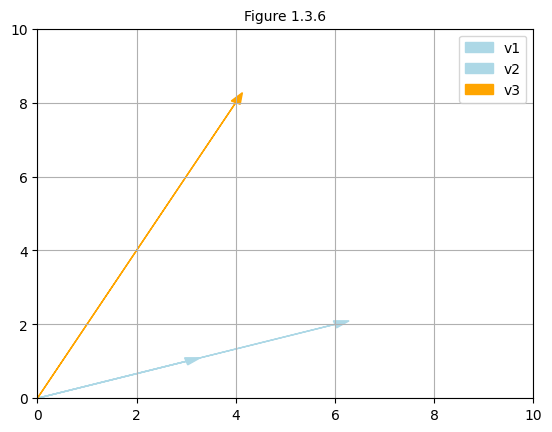
\includegraphics[width=5cm, height=4cm]{problem1.3.6} \\

How many solutions does the system

\begin{equation*}
x\vec{v_{1}} + y\vec{v_{2}} = v_{3}
\end{equation*}

have? Argue geometrically.
\end{problem}

\begin{solution}
Let $L$ be the line defined by the origin and $\vec{v_{3}}$. A linear combination of $\vec{v_{1}}$ and $\vec{v_{1}}$ can only intersect L at the origin, but not at the tip of $\vec{v_{3}}$. Thus there are no solutions to the system.
\end{solution}

\begin{problem}
Vectors $\vec{v_{1}}$, $\vec{v_{2}}$ and $\vec{v_{3}}$ are shown in the figure below. \\

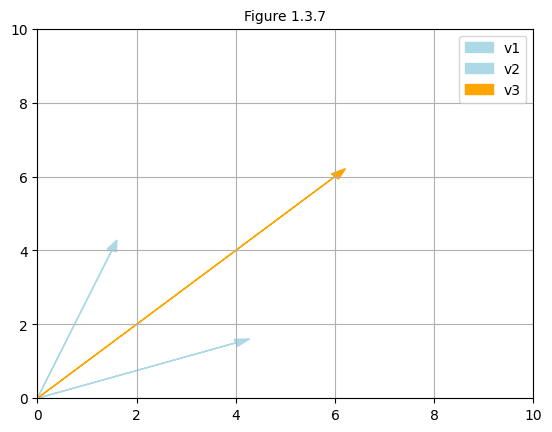
\includegraphics[width=5cm, height=4cm]{problem1.3.7} \\

How many solutions does the system

\begin{equation*}
x\vec{v_{1}} + y\vec{v_{2}} = v_{3}
\end{equation*}

have? Argue geometrically.
\end{problem}

\begin{solution}
The system has exactly one solution, because there is only one parallelogram with sides along vectors $\vec{v_{1}}$ and $\vec{v_{2}}$ and a vertex at the tip of $\vec{v_{3}}$. 
\end{solution}

\begin{problem}[1.3.9]
Write the system 

\begin{align*}
\begin{vmatrix}
x + 2y + 3z = 1 \\
4x + 5y + 6z = 4 \\
7x + 8y + 9z = 9
\end{vmatrix}
\end{align*}

in matrix form.
\end{problem}

\begin{solution}
\begin{align*}
\begin{pmatrix}
1 & 2 & 3 \\
4 & 5 & 6 \\ 
7 & 8 & 9 
\end{pmatrix}
\begin{pmatrix}
x \\ y \\ z
\end{pmatrix}
=
\begin{pmatrix}
1\\ 4 \\ 9
\end{pmatrix}
\end{align*}
\end{solution}

Compute the dot products in the following three problems (if the dot products are defined).

\begin{problem}[1.3.10] 
\begin{align*}
\begin{bmatrix}
1 \\ 2 \\ 3
\end{bmatrix}
\cdot
\begin{bmatrix}
1 \\ -2 \\ 1
\end{bmatrix}
\end{align*}
\end{problem}

\begin{solution}
\begin{align*}
&\begin{bmatrix}
1 \\ 2 \\ 3
\end{bmatrix}
\cdot
\begin{bmatrix}
1 \\ -2 \\ 1
\end{bmatrix} \\
&= (1 * 1) + (2 * -2) + (3 * 1) \\
&=1 - 4 + 3 \\
&= 0
\end{align*}

\end{solution}

\begin{problem}[1.3.11]
\begin{align*}
\begin{bmatrix}
1 & 9 & 9 & 7
\end{bmatrix}
\cdot
\begin{bmatrix}
6 \\ 6 \\ 6
\end{bmatrix}
\end{align*}
\end{problem}

\begin{solution}
There is no solution, since the row vector and column vector have a different number of components. The dot product of two vectors can only be computed if the two vectors have the same number of components.
\end{solution}

\end{document}